\chapter{Theoretischer Teil}

\section{Virtuelle Maschinen} 
Die hier gesammelten Informationen wurden bei IBM\cite{vm} recherchiert. IBM ist mit RedHat ein Vorreiter auf diesem Bereich.\\
Als virtuelle Maschine bezeichnet man die Emulation einer physischen Maschine.
Durch Virtualisierung ist es möglich mehrere dieser \ac{VM}s auf einer Hardwaremaschine laufen zu lassen.
So können Maschinen mit verschiedenen Hardware-Eigenschaften, Betriebssystemen und Applikationen sich die zur Verfügung stehenden Ressourcen teilen, so dass sparsamer gearbeitet werden kann.

\subsection{Wie Virtualisierung funktioniert}
Eine \ac{VM} kann nicht direkt mit der ihr zugrunde liegenden Hardware kommunizieren. 
Sie benötigt dafür einen sogenannten Hypervisor.
Der Hypervisor ist eine dünne Softwareschicht, die auf dem Host läuft, und über die physische Ressourcen den einzelnen \ac{VM}s zugewiesen werden können.

Hypervisor lassen sich in zwei Typen einordnen:
\begin{itemize}
    \item Typ 1 \\ 
            Der Hypervisor wird direkt auf dem bare metal Server installiert, womit eine geringe Latenz und hohe Sicherheit garantiert werden.
    \item Typ 2\\
            Zwischen dem bare metal Server und dem Hypervisor ist eine \ac{OS} Schicht installiert. 
            Dieser Typ findet hauptsächlich bei Endnutzern Verwendung, die auf ihrer lokalen Maschine Virtualisierung betreiben wollen, zum Beipsiel um eine \ac{VM} zu testen bevor sie auf der eigentlichen Virtualisierungsumgebung ausgerollt wird.
            Durch die zusätzliche \ac{OS} Schicht ist die Latenz höher als beim ersten Typen.
\end{itemize}

Durch die Unabhängigkeit von der Hardware ist es möglich die \ac{VM}s problemlos zwischen verschiedenen Hosts zu verschieben. \\

\subsection{Vorteile von Virtuellen Maschinen}
Da sich durch diese Technologie mehrere Applikationen und Maschinen dieselben Ressourcen teilen können, ist das Arbeite mit \ac{VM}s deutlich Ressourcenschonender und effizienter als das Arbeiten mit klassischen hardware-Servern.
Durch den geringeren Verbrauch von Mitteln zahlt sich das Einsetzen auch aus finanzieller Sicht aus.
Des weiteren können die Server deutlich agiler gemanaged und vor allem auch schneller bereitgestellt werden.
Die Agilität führt auch dazu, dass Downtimes bei Umzügen oder Updates der Umgebungen reduziert werden.


\section{Container}
Die Informationen aus diesem Absatz stammen von Google\cite{containers}, einem der größten Innovatoren auf dem Bereich der Containertechnologien.
\subsection{Was ist ein Container?}
Unter einem Container verstehen wir ein vollständiges Paket, dass alle Bausteine enthält um eine bestimmt Applikation zu deployen.
Da alle Bestandteile in Ihm vereint sind ist das Deployment der Anwendung so komplett unabhängig von der zugrundeliegenden Umgebung, was den Prozess vereinfacht und verzulässiger macht.
Außerdem erlaubt es diese Isolierung der Applikation auch eine klare Grenze zwischen Anwendungsentwickler und Betrieb zu ziehen:
Der Entwickler kann sich darauf verlassen, dass seine Software immer unter den exakt gleichen Bedingungen ausgeführt wird, mit den gleichen Abhängigkeiten, den gleichen Software-Versionen und auf dem gleichen Betriebssystem.
\\
Der IT-Betrieb hingegen kann sich darauf verlassen, dass ein Container sich immer gleich verhält. 
Er muss für verschiedene Anwendungen keine unterschiedlichen Betriebssysteme und Software-Versionen installieren, sondern muss nur den Container managen.
\\
Container können also, wie auch \ac{VM}s, als isolierte Umgebungen betrachtet werden, sie sind allerdings deutlich kleiner.

\subsection{Vorteile von Containern}

Container virtualisieren auf \ac{OS}-Level und auf dem gleichen Kernel wie das \ac{OS}.
Dadurch können sie deutlich schneller gestartet werden und haben einen deutlich kleineren Overhead als \ac{VM}s, da sie kein komplett funktionsfähiges Betriebssystem benötigen um zu laufen.
Der komplette Speicherplatz-, CPU- und Arbeitsspeicher-Verbrauch des \ac{OS} wird somit an Ressourcen auf dem Host-System eingespart.

\subsubsection{Gleichbleibende Umgebung}
Da in dem Container immer von einer gleichbleibenden Umgebung ausgegangen werden kann, wird die Produktivität der einzelnen Entwicklern deutlich gestiegert.
Diese müssen sich, durch die Verwendung von Container-Technologien, nicht länger mit unterschiedlichen Umgebungsbedingungen auseinandersetzen und können sich auf das entwickeln neuer Featuren konzentrieren.

\subsubsection{Auf jeden System ausführbar}
Container sind auf fast jedem System ausführbar. 
Ob Linux, Mac, Windows, \ac{VM}s, Datacentern oder Bare Metal.
Dies wird nicht zuletzt durch das sehr populäre Docker Image Format gewährleistet, das überall sehr verbreitet ist. 

\subsubsection{Isolation}
Arbeitsspeicher, CPU und Speicher sind auf Betriebssystemebene virtualisiert und somit bis zu einem gewissen Level vom Rest des Systems abgegrenzt. 
Die Isolation ist jedoch weniger stark als bei \ac{VM}s.


\section{Vergleich von Virtuellen Maschinen und Containern}

Beide Technologien haben ähnliche Ziele: \\
Höhere Schnelligkeit und Agilität beim Bereitstellen von Software, geringere Downtimes und Einspraung von Ressourcen. \\
Durch die unterschiedliche Herangehensweise hat jede Technologie andere Anwendungsbereiche als Ziel, sowie andere Stärken.
Die zusätzliche \ac{OS}-Schicht, in Abbildung \ref{fig:comparison_vm_container} dargestellt, bringt zwar einen deutlich größeren Overhead mit sich, dafür aber auch bessere abgrenzen der einzelnen Applikationen voneinander.
Die wichtigsten Unterschiede sind in Tabelle \ref{table:comparison_vm_container} noch einmal zusammengefasst. 

\begin{table}
        \centering
        \begin{tabular}{ | p{0.25\textwidth} | p{0.25\textwidth} | p{0.25\textwidth} | }
        Kategorie & Virtuelle Maschine & Container \\
        \hline \\
        Startup-Zeit & Im Minuten Bereich & Millisekunden bis Sekunden \\
        Performance & Großer Overhead, dadurch reltiv langsam & Kleiner Overhead, sehr schnell\\
        Operating System & Jede \ac{VM} kann auf einem unterschiedlichen \ac{OS} laufen & Alle Container teilen sich das \ac{OS} des Hosts \\
        Operations & Anpassungen müssen auf den \ac{VM}s vorgenommen werden. Unterschiedliche Maschinen, welche dieselbe Applikation bereitstellen können sich somit trotzdem unterscheiden. & Durch die deklarative Natur der Containertechnologien müssen keine Administratoren den Containern arbeiten. Anpassungen werden ausschließlich in den Images und Dockerfiles vorgenommen. Der Administrative Aufwand ist sehr gering. \\
        \end{tabular}
        \caption{Unterschiede von VM's und Containers}
        \label{table:comparison_vm_container}
\end{table}

\begin{figure}
        \caption{Vergleich von \ac{VM}s und Containern\cite{vm_vs_container}}
        \centering
        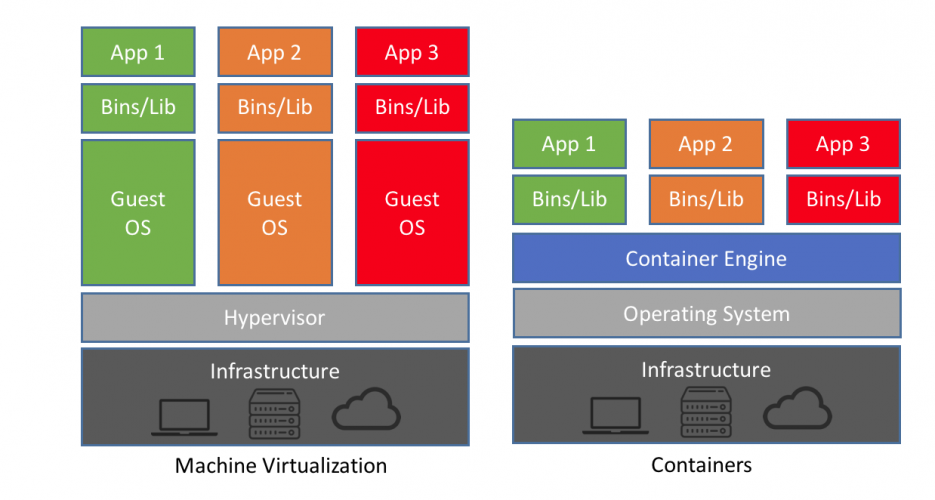
\includegraphics[width=0.8\textwidth]{bilder/comparison_vm_container.png}
        \label{fig:comparison_vm_container}
\end{figure}

\section{Kata-Runtime}


\section{Kubernets}

\section{Ansible}

\section{Helm}

\section{Backup (Stash)} \todo{Update if switching to other backup}